\chapter{Preliminary Results}\label{cap:preliminary-results}
\glsresetall

% =====================================================================
% SKELETON. Target: 10--14 pages.
%
% The tables below are PRE-FILLED from docs/status.md as of 2026-08-06, with
% the originating lab note given in each caption. Cross-check every number
% against its dated entry in docs/experiments/ before submitting; those files
% are append-only and authoritative, docs/status.md is a living summary.
%
% Reporting principle for this chapter: the negative calibration result and
% the tie with the prior art are REPORTED, not softened. They are what make
% the contribution claim in Chapter~\ref{cap:introduction} defensible, and a
% banca that finds them by asking will trust the rest of the document less.
% =====================================================================

This chapter reports what has been measured on the trained model to date. Each section
isolates one property with its own instrument: trajectory following
(Section~\ref{sec:res-ramp}), identity consistency across the trajectory
(Section~\ref{sec:res-identity}), absolute calibration (Section~\ref{sec:res-calibration}),
the emergence of the capability over training (Section~\ref{sec:res-dose}), a head-to-head
against the closest prior art (Section~\ref{sec:res-headtohead}), and the whole-face response
to the single axis (Section~\ref{sec:res-coactivation}). The negative calibration result and
the tie with the prior art are reported plainly rather than softened: they are what make the
contribution claim of Chapter~\ref{cap:introduction} defensible. Every number traces to the
dated laboratory note cited in its caption.

% =====================================================================
\section{Experimental Setup}\label{sec:res-setup}

% Checkpoint (100k steps, single RTX 3090), prompt bank size, seeds,
% frames per clip, intensity lists used. Point to the batch-eval harness so
% the numbers are reproducible.

All numbers below come from the released 100k-step checkpoint
(Section~\ref{sec:method-training}), generated on a single RTX~3090. Unless a table states
otherwise, evaluation uses the bank of 40 text prompts, three seeds ($42,43,44$), and
five-frame clips at $256\times384$, decoded at 25 denoising steps with classifier-free
guidance scale $8.0$. The ascending ramp commands the intensity list $(0,0.25,0.5,0.75,1.0)$;
the constant-list and permuted-list designs of Section~\ref{sec:method-evaluation} supply the
calibration and non-monotonic probes. Generation and scoring run through the
batch-evaluation harness, so every reported figure is reproducible from the same seeds and
configuration.

% =====================================================================
\section{Trajectory Following}\label{sec:res-ramp}

% Headline: control over the trajectory is real and robust at scale, and it
% is confirmed by an estimator that produced none of the training labels.
% The descending-ramp reversal near -1 is strong evidence that the model
% responds to the conditioning signal rather than to a fixed temporal prior.

\begin{table}[H]
    \centering
    \caption{Trajectory following, measured as Pearson correlation $r$ between commanded and detected AU12 intensity, with the per-condition sample size $n$.}
    \label{tab:res-ramp}
    \begin{tabular}{@{}lccc@{}}
        \toprule
        Condition & $n$ & py-feat AU12 $r$ & MediaPipe proxy $r$ \\
        \midrule
        Trained adaptor, ascending ramp  & $120$ & $0.774 \pm 0.212$ & $0.829 \pm 0.230$ \\
        Frozen backbone baseline         & $120$ & $-0.05 \pm 0.64$  & $-0.02 \pm 0.66$ \\
        Trained adaptor, descending ramp & $1$   & $-0.98$           & not measured \\
        Trained adaptor, permuted list   & $90$  & $0.385 \pm 0.505$ & $0.46 \pm 0.45$ \\
        \bottomrule
    \end{tabular}\\[4pt]
    {\footnotesize Source: prepared by the author. Lab notes 2026-07-08 and 2026-07-14. The baseline MediaPipe proxy is computed on only the 44/120 clips with a valid measurement, which flatters it; the descending-ramp MediaPipe proxy was not measured (that run predates MediaPipe scoring).}
\end{table}

Table~\ref{tab:res-ramp} establishes that trajectory following is real and robust at scale.
On the ascending ramp the trained adaptor reaches $r=0.774\pm0.212$ (median $0.86$, with
$87\%$ of clips above $0.5$), against a frozen-backbone baseline indistinguishable from zero.
The result is corroborated by the MediaPipe proxy ($r=0.829$), an estimator that produced none
of the training labels, so the effect is not an artefact of the py-feat pipeline. The
descending-ramp reversal to $r=-0.98$ shows the model tracks the commanded signal rather than a
fixed temporal prior. The permuted-list drop to $r=0.385\pm0.505$ is a scope statement rather
than a failure: the conditioning is genuinely per-frame, but the temporal prior resists
non-monotonic trajectories, for which the ramp-only training data offers no support.

% Interpretation point worth making explicitly: the permuted-list result
% (0.385) shows the conditioning is genuinely per-frame, but that the
% temporal prior resists non-monotonic trajectories, for which the training
% data contains no support. This is a scope statement, not a failure.

% =====================================================================
\section{Identity Consistency}\label{sec:res-identity}

% The measurement that isolates the sequence-native claim. Note the
% qualitative asymmetry that matters as much as the number: the baseline's
% faces were undetectable in 57% of samples, so its 0.85 is computed on the
% easier remainder and flatters it.

\begin{table}[H]
    \centering
    \caption{Frame-to-frame face-embedding cosine similarity within a generated clip. The adjacent-frame minimum, the worst single transition, is the quantity the head-to-head comparison turns on.}
    \label{tab:res-identity}
    \begin{tabular}{@{}lccc@{}}
        \toprule
        Condition & Mean cosine & Adjacent-frame min. & Face detected \\
        \midrule
        Trained adaptor          & $0.92 \pm 0.05$ & $0.877 \pm 0.086$ & $120/120$ \\
        Frozen backbone baseline & $0.85$          & $0.794 \pm 0.152$ & $43\%$ \\
        \bottomrule
    \end{tabular}\\[4pt]
    {\footnotesize Source: prepared by the author. Lab note 2026-07-14, facenet-VGGFace2 embeddings. The baseline's faces were undetectable in 57\% of samples, so its cosines are computed on the easier remainder.}
\end{table}

Table~\ref{tab:res-identity} isolates the sequence-native claim. Within a generated clip the
trained adaptor holds a frame-to-frame identity cosine of $0.92\pm0.05$ and, more tellingly, an
adjacent-frame minimum of $0.877\pm0.086$ against the baseline's $0.794\pm0.152$; the
adjacent-frame minimum is reported because the worst transition is the one a viewer notices, and
it is the quantity the head-to-head comparison turns on. The comparison is not quite symmetric:
the baseline's faces were undetectable in $57\%$ of samples, so its cosines are computed on the
easier detectable remainder and are flattered. Identity is measured here with a single embedding
network (facenet-VGGFace2); multi-model averaging with an ArcFace embedding is scheduled as
proposed work in Chapter~\ref{cap:schedule}.

% =====================================================================
\section{Absolute Calibration}\label{sec:res-calibration}

% NEGATIVE RESULT. Report it plainly and diagnose it.
%
% Finding: holding the commanded value constant across a clip and varying it
% between clips produces almost no change in detected intensity
% (\gls{cls} = 0.07; detected AU12 flat near 0.85 for every commanded level
% at or above 0.1). The same commanded value of 0.0 renders as 0.54 inside a
% ramp and 0.79 in a constant clip.
%
% Consequence: the control is RELATIVE and contextual, not absolute. The
% conditioning commands a trajectory, not a value.
%
% Root cause: the training clips are onset-to-apex ramps only
% (Section~\ref{sec:method-data}), so the model never observed a constant
% intensity trajectory.
%
% This refutes H3 from Section~\ref{sec:hypotheses}. Say so in those words.

The calibration measurement is a negative result, and it is reported as one. Holding the
commanded value constant across a clip and varying it between clips produces almost no change in
detected intensity: the calibration score is $\gls{cls}=0.07$, and the detected AU12 sits flat
near $0.85$ for every commanded level at or above $0.1$. The context-dependence is stark: the
same commanded value of $0.0$ renders as $0.54$ inside an ascending ramp but $0.79$ in a
constant clip. The control is therefore \emph{relative and contextual}, not absolute: the
conditioning commands a trajectory, not a value. This refutes hypothesis H3 of
Section~\ref{sec:hypotheses}. The cause is in the training data, not the architecture: the
clips are onset-to-apex ramps only (Section~\ref{sec:method-data}), so the model never observed
a constant-intensity trajectory to calibrate against.

Three remedies are plausible and are carried as proposed work in Chapter~\ref{cap:schedule},
not as claims: augmenting the training set with constant- and permuted-intensity clips so the
model observes non-ramp trajectories; AU dropout with classifier-free guidance on the
expression condition \citep{wei2025magicface}; and label-distribution smoothing
\citep{varanka2024fineface}. None has been run.

% =====================================================================
\section{Training Drives the Capability}\label{sec:res-dose}

To confirm that trajectory following is learned rather than inherited from the frozen
backbone, the ascending-ramp evaluation was repeated at six checkpoints spanning the single
1k--100k training run (Figure~\ref{fig:dose}). Against an untrained baseline of $r=-0.05$,
control is already at $r=0.55$ by 1k steps and rises to a plateau near $0.85$ by 25k--50k, a
monotone trend over training (Spearman$(\text{step},r)=+0.60$) that the label-independent
MediaPipe proxy tracks. Per-prompt variance also shrinks as training proceeds (standard
deviation $0.43\to0.13$), so later training makes the control more consistent even after the
mean saturates.

\begin{figure}[t]
    \centering
    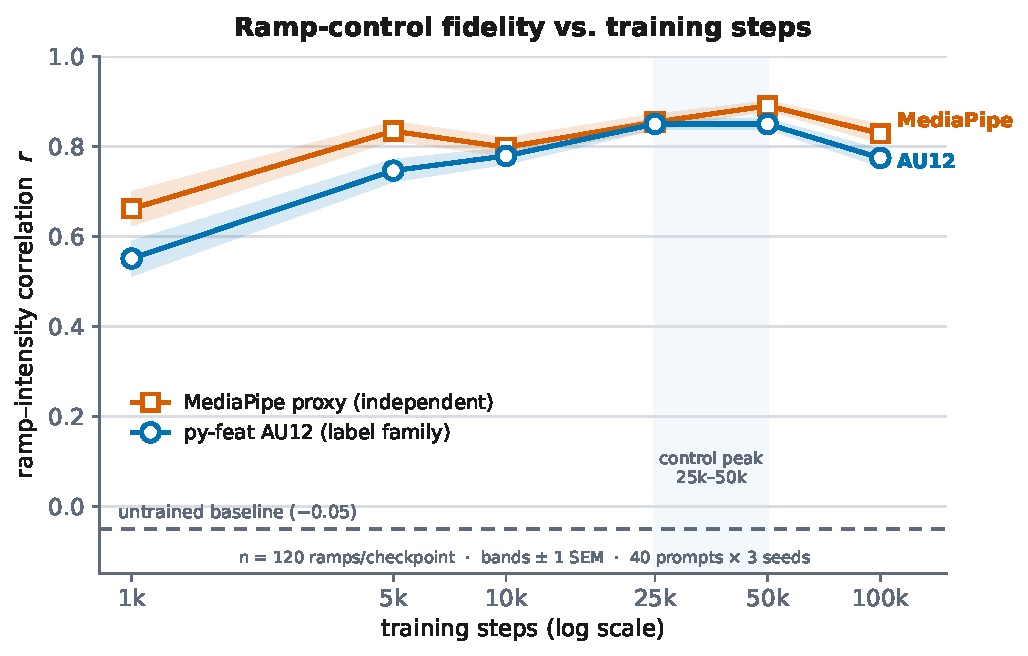
\includegraphics[width=0.78\textwidth]{images/2026-08-11-dose-response.pdf}
    \caption{Ramp-control fidelity against training steps, at six checkpoints of the single
    training run ($n=120$ ramps per checkpoint, bands $\pm1$ SEM). Both the py-feat AU12
    correlation and the label-independent MediaPipe proxy rise and plateau. Lab note 2026-08-11.}
    \label{fig:dose}
\end{figure}

A caveat follows from the curve: the released 100k checkpoint is mildly past-peak for ramp
following ($r=0.774$ against $0.850$ at 50k; Welch $t\approx3.4$), and every headline number
in this chapter comes from it. Re-evaluating at a 25k--50k checkpoint is therefore a cheap
improvement, noted as proposed work in Chapter~\ref{cap:schedule}.

% =====================================================================
\section{Comparison with the Closest Prior Art}\label{sec:res-headtohead}

% The single most important external comparison in the proposal
% (lab note 2026-07-21, n=120 matched prompts). The verdict is mixed and
% must be presented as mixed.

\begin{table}[H]
    \centering
    \caption{Head-to-head against \citet{varanka2024fineface} under matched prompts and intensity levels ($n=120$). Higher is better in every column.}
    \label{tab:res-headtohead}
    \begin{tabular}{@{}lccc@{}}
        \toprule
        System & Ramp $r$ (py-feat) & Calibration (\gls{cls}) & Identity (adjacent min.) \\
        \midrule
        FineFace, independent stills & $0.786$ & $0.50$ & baseline \\
        This work, one clip          & $0.774$ & $0.07$ & $+0.12$ \\
        \bottomrule
    \end{tabular}\\[4pt]
    {\footnotesize Source: prepared by the author. Lab note 2026-07-21.}
\end{table}

% Read the table out loud in the text, in this order:
%   1. Ramp following is a TIE (FineFace marginally ahead, and further ahead
%      on the MediaPipe proxy: 0.88 vs 0.83).
%   2. FineFace WINS absolute calibration decisively.
%   3. This work wins cross-frame identity, modestly but consistently
%      (63--68% of prompts, roughly 2.5x lower variance).
% Therefore the defensible contribution is the sequence-native formulation
% and the measurement protocol, NOT superior expression control. State this
% conclusion explicitly here so that Cap01 and Cap06 can rely on it.

Table~\ref{tab:res-headtohead} is the single most important external comparison, and its
verdict is mixed. Read in order: first, ramp following is a tie. FineFace is marginally ahead on
py-feat ($0.786$ against $0.774$) and further ahead on the MediaPipe proxy ($0.88$ against
$0.83$), a difference within noise. Second, FineFace wins absolute calibration decisively
($\gls{cls}=0.50$ against $0.07$), consistent with the ramp-only limitation of
Section~\ref{sec:res-calibration}. Third, this work wins cross-frame identity, modestly but
consistently: the adjacent-frame minimum is higher on $63$--$68\%$ of prompts, with roughly
$2.5\times$ lower variance. The conclusion, which Chapters~\ref{cap:introduction}
and~\ref{cap:schedule} rely on, is therefore explicit: the defensible contribution is the
sequence-native formulation and the measurement protocol, not superior expression control.

% =====================================================================
\section{Whole-Face Response}\label{sec:res-coactivation}

A single scalar axis invites the question of what \emph{else} it moves. Re-scoring the
ascending-ramp clips for all twenty py-feat action units, cross-checked against an
independent estimator (LibreFace) and against face-mesh geometry, shows that the axis drives
a coherent smile expression rather than an isolated muscle (Figure~\ref{fig:coactivation}).
The commanded AU12 and the Duchenne cheek raiser AU6 co-activate strongly and are
model-induced (both Spearman $r>0.87$, and significant at $q<0.05$ against the frozen
baseline); mouth-opening units (AU25/26) rise while mouth-closing and frowning units (AU23,
AU17, AU15) fall. Brow units sit near zero on py-feat, although the independent detectors
reveal a subtle brow entanglement that py-feat underreports, and the cross-check exposes one
py-feat artefact (AU20, which the independent estimator contradicts). This is a feature and a
limitation at once: the rendered change is a natural, coherent expression, but AU12 is not
isolable. It is the empirical basis for the multi-AU extension proposed in
Chapter~\ref{cap:schedule}.

\begin{figure}[t]
    \centering
    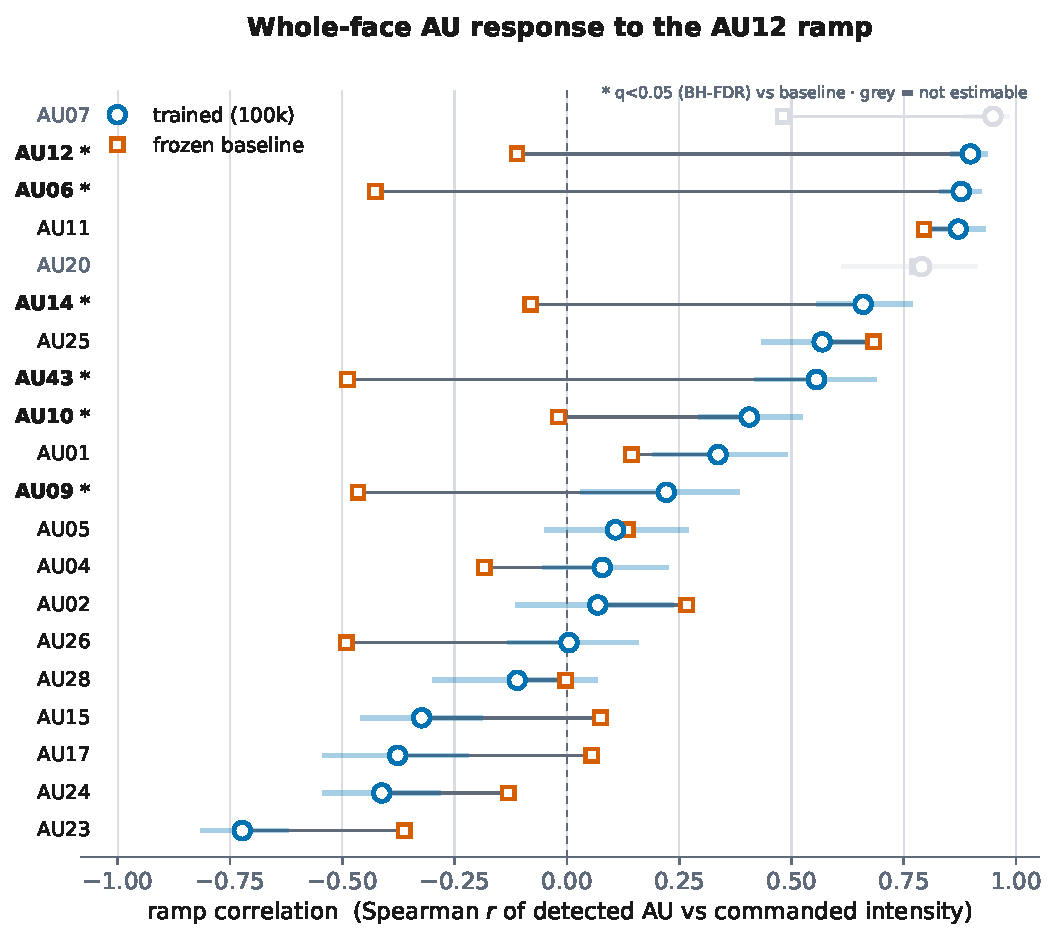
\includegraphics[width=0.72\textwidth]{images/2026-08-25-au-coactivation-profile.pdf}
    \caption{Per-action-unit response to the AU12 ramp (Spearman $r$, trained adaptor versus
    frozen baseline). The smile cluster (AU12, AU6, AU25) co-activates and the mouth-closing
    units (AU23, AU17) anti-correlate, while brow units are near zero. Asterisks mark units
    significantly modulated by training ($q<0.05$, Benjamini--Hochberg). Lab note 2026-08-25.}
    \label{fig:coactivation}
\end{figure}

% =====================================================================
\section{Qualitative Results}\label{sec:res-qualitative}

% Suggested figures (place the exported frames under images/):
%   1. One ramp: frames at commanded 0.0 to 1.0, trained vs frozen baseline.
%   2. Side-by-side with FineFace stills at matched levels, to make the
%      identity drift visible rather than merely tabulated.
%   3. A failure case. Include one; it buys credibility.

Figure~\ref{fig:qualitative} shows one ascending ramp for a single prompt and seed, with the
trained adaptor above and the frozen backbone below. With the adaptor, the commanded intensity
drives a smile that intensifies across the clip while identity and framing stay consistent;
without it, the same commanded trajectory leaves the generated portrait essentially unchanged.
The trained row also makes visible the domain shift noted in Section~\ref{sec:res-threats}: the
adaptor pulls the output toward the lab-recorded \gls{mead} appearance it was trained on.

\begin{figure}[t]
    \centering
    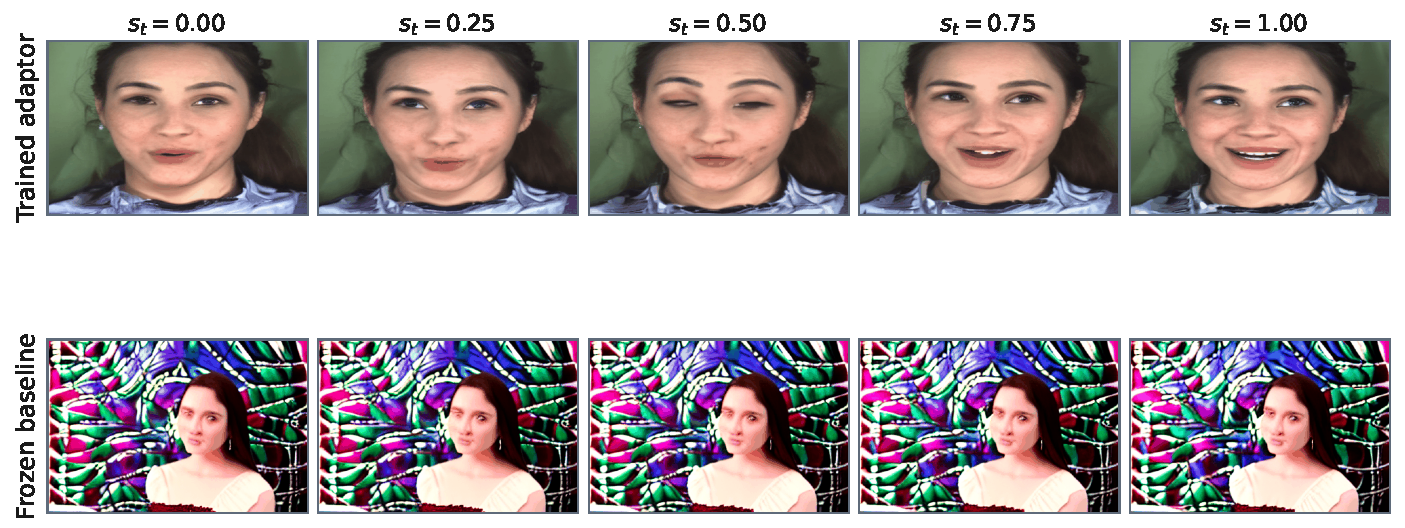
\includegraphics[width=\textwidth]{images/2026-08-25-qualitative-ramp.pdf}
    \caption{One ascending ramp (prompt: ``a portrait photograph of a young woman, frontal
    view, neutral background''; seed 42), with commanded intensity $s_t$ increasing left to
    right. Top: the trained adaptor, where the smile intensifies while identity is preserved
    across frames. Bottom: the frozen backbone under the same seed, left unchanged by the
    commanded trajectory.}
    \label{fig:qualitative}
\end{figure}

% =====================================================================
\section{Threats to Validity}\label{sec:res-threats}

\begin{itemize}
    \item \textbf{Label--evaluation circularity.} py-feat provides both the training labels and the primary metric. Mitigated by the independent MediaPipe measurement (Section~\ref{subsec:eval-circularity}), which agreed, but not eliminated.
    \item \textbf{Demographic bias.} Ramp $r$ is $0.83$ for female prompts against $0.71$ for male prompts. The prior art shows the opposite skew (FineFace: $0.82$ male against $0.77$ female), which localises the cause to the \gls{mead} training distribution rather than to AU-conditioned generation in general.
    \item \textbf{Lab-domain training data.} A single dataset, a single emotion category, frontal views, controlled lighting. Generalisation to in-the-wild portraits is untested.
    \item \textbf{Single control axis.} Only AU12 is conditioned. The whole-face analysis (Section~\ref{sec:res-coactivation}) shows the axis co-activates the entire smile cluster and cannot isolate a single unit; the prior art controls twelve action units and their combinations. A multi-AU axis is proposed in Chapter~\ref{cap:schedule}.
    \item \textbf{Single training run.} One seed, one checkpoint; no variance estimate over training runs.
\end{itemize}
